\documentclass{article}

\usepackage{algorithm,algpseudocode}
\usepackage{a4wide,amsmath,amssymb,fancyhdr,graphicx,tabularx,xspace}

%------------------------------------------------------------------------------
\newcommand{\course}{Advanced Algorithms}
\newcommand{\coursenumber}{2IMA10}
\newcommand{\courseyear}{Fall 2017}
%------------------------------------------------------------------------------
\pagestyle{fancy}
\chead{}
\lhead{TU Eindhoven}
\rhead{\course\ (\coursenumber) --- Homework Exercises, \courseyear}
\cfoot{\thepage}
\lfoot{}
\rfoot{}
%------------------------------------------------------------------------------

%to include IPE/pdf correctly
\expandafter\ifx\csname pdfoptionalwaysusepdfpagebox\endcsname\relax\else
\pdfoptionalwaysusepdfpagebox5
\fi


\newcommand{\Reals}{{\Bbb R}}
\newcommand{\Nats}{{\Bbb N}}
\newcommand{\Ints}{{\Bbb Z}}

\newcommand{\C}{\ensuremath{\mathcal{C}}}
\newcommand{\E}{\ensuremath{\mathcal{E}}}
\newcommand{\F}{\ensuremath{\mathcal{F}}}
\newcommand{\G}{\ensuremath{\mathcal{G}}}
\newcommand{\U}{\ensuremath{\mathcal{U}}}

\newcommand{\tree}{\ensuremath{\mathcal{T}}}
\newcommand{\node}{\nu}
\newcommand{\lchild}{\mathrm{lc}}
\newcommand{\rchild}{\mathrm{rc}}
\newcommand{\size}{\mathit{size}}
\newcommand{\leaf}{\mu}
\newcommand{\mylist}{{\cal L}}
\newcommand{\myroot}{\mathit{root}}
\newcommand{\key}{\mathit{key}}
\newcommand{\bd}{\partial}

\newcommand{\myopt}{\mbox{{\sc opt}}\xspace}
\newcommand{\lb}{\mbox{{\sc lb}}\xspace}
\newcommand{\loadb}{{\sc Load Balancing}\xspace}

\newcommand{\vc}{{\sc Vertex Cover}\xspace}
\newcommand{\wvc}{{\sc Weighted Vertex Cover}\xspace}
\newcommand{\wsetc}{{\sc Weighted Set Cover}\xspace}
\newcommand{\tsp}{{\sc TSP}\xspace}
\newcommand{\mst}{{\sc MST}\xspace}

\newcommand{\eps}{\varepsilon}
\newcommand{\ol}{\overline}
\renewcommand{\leq}{\leqslant}
\renewcommand{\geq}{\geqslant}

\newcommand{\pr}[1]{\Pr[#1]}
\DeclareMathOperator{\expectation}{E}
\newcommand{\expt}[1]{\expectation[#1]}
\newcommand{\events}[1]{\mbox{Events}(#1)}
\newcommand{\rank}{\mathit{rank}}
\newcommand{\result}{\mathit{result}}
\newcommand{\piv}{\mathrm{piv}}
\newcommand{\myexp}{\mathrm{exp}}
\newcommand{\best}{\mathrm{best}}
\newcommand{\worst}{\mathrm{worst}}
\newcommand{\dest}{\mathit{dest}}
\newcommand{\dist}{\mathit{distance}}
\newcommand{\weight}{\mathit{weight}}
\newcommand{\mylength}{\mathit{length}}
\newcommand{\length}{\mathit{length}}
\newcommand{\mymid}{\mathrm{mid}}
\newcommand{\alg}{{\sc Alg}\xspace}

\newcommand{\start}{\mathit{start}}
\newcommand{\myend}{\mathit{end}}
\newcommand{\free}{\mathit{free}}
\newcommand{\true}{{\sc True}\xspace}
\newcommand{\false}{{\sc False}\xspace}

\newcommand{\etal}{{\emph{et al.}\xspace}}

\newcommand{\io}{{\sc i/o}\xspace}
\newcommand{\ios}{{\io}s\xspace}
\newcommand{\lru}{{\sc lru}\xspace}
\newcommand{\sort}{\mbox{\sc Sort}}

%------------------------------------------------------------------------------
% Theorem-Like Environments
%------------------------------------------------------------------------------
\newtheorem{defin}{Definition}
  \newenvironment{mydefinition}{\begin{defin} \sl}{\end{defin}}
\newtheorem{theo}[defin]{Theorem}
  \newenvironment{mytheorem}{\begin{theo} \sl}{\end{theo}}
\newtheorem{lem}[defin]{Lemma}
  \newenvironment{mylemma}{\begin{lem} \sl}{\end{lem}}
\newtheorem{propo}[defin]{Proposition}
  \newenvironment{myproposition}{\begin{propo} \sl}{\end{propo}}
\newtheorem{coro}[defin]{Corollary}
  \newenvironment{corollary}{\begin{coro} \sl}{\end{coro}}

\newenvironment{myproof}{\emph{Proof.}}{\hfill $\Box$ \medskip\\}

%------------------------------------------------------------------------------
\newcounter{rcounter}
\newenvironment{rlist}%
{\begin{list}{\setnr-\arabic{rcounter}}{\usecounter{rcounter}}}{\end{list}}
\newcounter{rcountermem}
%------------------------------------------------------------------------------

\title{Advanced Algorithm Assignment II}
\author{Freerk Hendrik Oudman, Pieter Jacob van der Perk, Weizhou Xing}
\date{\today}

\begin{document}

\maketitle

%------------------------------------------------------------------------------
\section*{Homework Exercises on I/O-Efficient Algorithms}
%------------------------------------------------------------------------------
The maximum number of points for all exercises is~30.
The grade for this homework set is: (number of scored points)/3.

%------------------------------------------------------------------------------
\newcommand{\setnr}{IO.I}
\subsection*{Exercise Set I/O-Efficient I}
%------------------------------------------------------------------------------
\begin{rlist}

\item ($1$ point)
    Suppose you have three search algorithms on a very large data set consisting of $n=10^9$ elements: one algorithm performs $\lceil \log_2 (n/B)\rceil$ \ios, one performs $\lceil \log_B n \rceil$ \ios, and one performs 20~\ios. Which one would you use in practice? Explain your answer by considering the number of \ios of the three algorithms for a realistic value of~$B$.
    
    \textbf{Answer:}
    
    There are three circumstances where one of these algorithms beats the other two in performance. We need to compare the performance of every two algorithm to find the boundaries of $B$.
    \begin{enumerate}
        \item[(i)]
            \begin{align*}
                &\lceil \log_2 (n/B)\rceil < 20 \\
                &\Longrightarrow \frac{n}{B} < 2^{20} \\
                &\Longrightarrow B_1 > \frac{n}{2^{20}} = \frac{10^9}{2^{20}} = \frac{10^9}{1024^2} \approx \frac{10^9}{10^6} = 10^3
            \end{align*}
        \item[(ii)]
            \begin{align*}
                &\lceil \log_2 (n/B)\rceil < \lceil \log_B n \rceil\\
                &\Longrightarrow \frac{\log_{10}(n/B)}{\log_{10}2} < \frac{\log_{10}n}{\log_{10}B} \\
                &\Longrightarrow \frac{9-\log_{10}B}{\log_{10}2} < \frac{9}{\log_{10}B} \\
                &\textrm{Let $x$ denote } \log_{10}B\\
                &\Longrightarrow \frac{9-x}{\log_{10}2} < \frac{9}{x} \\
                &\Longrightarrow 9x-x^2 < 9 \cdot \log_{10}2\\
                &\textrm{Applying abc-formula:}\\
                & x > 8.7 \vee x < 0.3\\
                & B_2 > 10^{8.7} \textrm{  or  } B_2 < 10^{0.3}
            \end{align*}
        \item[(iii)]
            \begin{align*}
                &\lceil \log_B n \rceil < 20\\
                &\Longrightarrow B > n^{\frac{1}{20}}\\
                &\Longrightarrow B_3 > 10^{9 \cdot \frac{1}{20}} \approx 10^{1/2} \approx 4\\
            \end{align*}
    \end{enumerate}
    For a realistic \io, the size of block should lie in range $10^3$ to $10^4$. Thus, the algorithm which performs $\lceil \log_B n \rceil$ \ios is the most optimal.
\item ($2$ point)
    Let $A[0..n-1]$ be a sorted array of $n$ numbers, stored in blocks in the natural way: $A[0..B-1]$ is the first block, $A[B..2B-1]$ is the second block, and so on. Consider the following four statements about the number of \ios when we do a binary search on~$A$.
    \begin{enumerate}
        \item[(I)]
            The number of \ios is $\Theta(n/B)$.
        \item[(II)]
            The number of \ios is $\Theta(\log_2 (n/B))$.
        \item[(III)]
            The number of \ios is $\Theta(\log_B(n))$.
        \item[(IV)]
            The number of \ios is $\Theta(\log_2 n)$.
    \end{enumerate}
    Which of these four statements is true? Briefly explain your answer. \emph{Note:} You only have to argue that the statement you choose is true, not that the others are false. (That follows automatically.)
    
    \textbf{Answer:}
    The second statement is true: The number of \ios is $\Theta(\log_2 (n/B))$.\\
    This can be written as $\Theta(\log_2n-\log_2B)$. This performance can be interpreted as that in the first few binary searchings, we need to perform \ios every time because numbers are far from each other (yellow blocks in Figure \ref{fig:bs}. However, after a few times of searches, all the number that we need to compare can be reached within one single \io block so no more \ios is needed (red block in Figure \ref{fig:bs}).
    %\begin{tikzpicture}
    %\draw (0,-2) -- (4,-2);
    %\end{tikzpicture}
    \begin{figure}[h]
        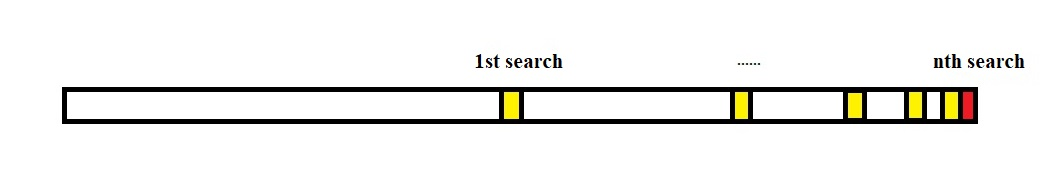
\includegraphics[width=\linewidth]{figs/I_2.jpg}
        \caption{Binary search, Yellow shows block, red shows last block}
        \label{fig:bs}
    \end{figure}

\item ($2$ points)
    Consider the algorithm from the Course Notes that computes the average value in an $m\times m$ array~$A$ column by column, for the case where $A$ is stored in row-major order. In the Course Notes it was stated (on page~43) that the algorithm performs $n$~\ios, where $n := m^2$ is the total size of the array. The reason is that whenever we need a new entry from the array, we have already evicted the block containing that entry. This is true when the Least-Recently-Used replacement policy is used and when $m > M/B$, but it is not immediately clear what happens when some other replacement policy is used.
    
    Prove that when $m>2M/B$, then \emph{any} replacement policy will perform $\Omega(n)$~\ios.
    
    \textbf{Answer1:}
    To proof that \emph{any} replacement policy will perform $\Omega(n)$~\ios. We have to proof that the optimal policy performs $\Omega(n)$~\ios. The MIN (Long Forward Distance) is a optimal replacement policy.
    
    Computing the average value in an $m\times m$ array~$A$ column by column in array which is stored in row-major order will yield a block for each row in the column. When $m>M/B$ not all blocks of one column fit into the memory, so for some blocks we have to perform one \io per entry. The MIN pattern would fill up the memory $M$ with the first $M/B-1$ entries of a column and swap all other entries of the column one by one. This gives $(M/B-1)(m/B)+(m-(M/B-1))m$. Since $m>2M/B \implies M/B < \frac{1}{2}m$, we get $(M/B-1)(m/B)+(m-(M/B-1))m > (M/B-1)(m/B)+\frac{1}{2}m^2 > \frac{1}{2}m^2 = \Omega(n)$ \ios.
    
    \textbf{Answer2:}
    Consider the algorithm uses \lru and have $2M$ memory. When it computes the average value of a matrix of size $m*m$, $m>2M/B$. we already proved that it will use $m*m=n$ \ios.
    From Theorem 5.3:
    $$\textrm{\sc Min}(\textrm{\alg}, M) > \frac{1}{2} \cdot \textrm{\lru}(\textrm{\alg}, 2M)$$
    $$\textrm{\sc Min}(\textrm{\alg}, M) > \frac{1}{2} \cdot n = \Omega(n)$$
    Since {\sc Min} is the optimal replacement policy, we them prove that any replacement policy will perform $Omega(n)$~\ios.
        
    %Computing the average value in an $m\times m$ array~$A$ column by column in array which is stored in row-major order. Will yield a block for each row in the column. When $m>2M/B$ yields that the blocks in each column is bigger then $2M$. The MIN pattern would fill up the memory $M$ with the first $M/B-1$ columns and swap the last entry with a new row. This would yield $n - (M/B -1) \cdot (m-1)$ \ios. Which is $\Omega(n)$~\ios.
    
    
    %Note wrong: !! 
    %From theorem 5.3 in the course notes it can be stated that $2 \cdot $MIN(Alg,$M$) $>$ %LRU(Alg,$2M$). 
    %So we have to proof that LRU(Alg,$2M$) performs $\Omega(n)$~\ios. TODO take proof from %book. Hence if LRU(Alg,$2M$) performs  $\Omega(n)$~\ios 


\item ($1+2\frac{1}{2}+2\frac{1}{2}$ points)
    Let $X[0..n-1]$ and $Y[0..n-1]$ be two arrays of $n$ numbers, where $n \gg M \gg B$. Suppose we have a function $f:\Reals^2\rightarrow \Reals$ and we want to compute $\min \{ f(X[i],Y[j]) : 0\leq i <n \mbox{ and } 0\leq j <n \}$. If we have no other information about $f$, then the only thing we can do is compute $f(X[i],Y[j])$ for all pairs $i,j$ with $0\leq i <n$ and $0\leq j <n \}$. A simple way to do this is using the following algorithm.
    %--------------------------------------------------------------------------------------------
    \begin{quotation}
    \noindent
    \emph{FindMin}$(X,Y)$ \\[-5mm]
    \begin{algorithmic}[1]
        \State $z \gets +\infty$
        \For{$i\gets 0$ \textbf{to} $n-1$}
           \For{$j\gets 0$ \textbf{to} $n-1$}
                \State $z \gets \min ( z, f(X[i],Y[j]) )$
           \EndFor
        \EndFor
        \State \Return $z$
    \end{algorithmic}
    \end{quotation}
    %--------------------------------------------------------------------------------------------
    \begin{enumerate}
        \item[(i)]
            Analyze the number of \ios performed by \emph{FindMin}.
        \item[(ii)]
            Give a cache-aware algorithm that solves the problem using $O(n^2/(MB))$ \ios, and prove that your algorithms achieves the desired \io-bound.
            
            \emph{Hint:} Partition both $X$ and $Y$ smaller subarrays, and solve the problem for each pair of subarrays separately.
        \item[(iii)]
            Give a cache-oblivious algorithm that solves the problem using $O(n^2/(MB))$ \ios, and prove that your algorithms achieves the desired \io-bound.
            
            \emph{Hint:} Use a recursive algorithm, and use a recurrence to analyze the \io-complexity. When writing the recurrence you should be precise about ``blocks sticking out'', similarly to what is done in the proof of Theorem~5.2. When solving the recurrence, you are allowed to ignore the blocks sticking out and work with a simplified recurrence.
    \end{enumerate}
    
    \textbf{Answer:}
    \begin{enumerate}
    	\item[(i)]
            The algorithm contains two for loops, one outer loop, lines 2-6 of the algorithm, and one inner loop, lines 3-5 of the algorithm. All data of $X$ is read and compared linear, therefore $X$ has a $O(\frac{n}{B})$ \io complexity.
            
            Data from $Y$ is however read in the inner loop. Since $n \gg M$, this data has to be read for every cycle of the outer loop. The complexity of $Y$ is therefore $n \cdot O(\frac{n}{B}) = O(\frac{n^2}{B})$ \ios, which gives a total \io complexity of $O(\frac{n^2}{B})$ \ios.
        \item[(ii)]
            I designed the following algorithm:
            
            \emph{CacheAwareFindMin}$(X,Y)$
            \begin{algorithmic}[1]
                \State $t \gets B \cdot \lfloor M / B \rfloor$ - B
                \State $z \gets +\infty$
                \For{$i\gets 0$ \textbf{to} $n/t$}
                    \State $X^* \gets X[i \cdot t : \min ((i+1) \cdot t - 1, n)]$
                    \For{$j\gets 0$ \textbf{to} $n/t$}
                        \State $Y^* \gets Y[j]$
                        \State $z \gets \min (z, FindMin(X^*, Y^*))$
                    \EndFor
                \EndFor
                \State \Return $z$
            \end{algorithmic}
            
            Instead of loading array entries one by one, we divide $X$ in bigger blocks that we load one by one in the internal memory. Lines 2-10 should be self-explaining. In order to minimize the \io complexity, we have to maximize $t = |X^*|$, so we get: $t = M$. To order with blocks sticking out, we divide by $B$, floor the result and then multiply by $B$ again. This way, we can take exact blocks from the external memory that will always fit into the internal memory. Since we need to reserve for one block of $Y$, we subtract $B$. 
            
            Again, the algorithm contains two for loops. All data of $X$ is linear read in the outer loop exactly one time, so we have again an \io complexity of $O(\frac{n}{B})$ \ios for $X$. The inner loop has again the same problem as before: since $n \gg M$, $Y$ has to be read once time for every cycle of the outer loop. This gives an \io complexity of $\frac{n}{t} \cdot O(\frac{n}{B}) = \frac{n}{B \cdot \lfloor M / B \rfloor - B} \cdot O(\frac{n}{B}) < \frac{n}{M} \cdot O(\frac{n}{B}) = O(\frac{n^2}{MB})$ \ios.
        \item[(iii)]
            I designed the following algorithm:
            
            \emph{CacheObliviousFindMin}$(X, i_1, i_2, Y)$
            \begin{algorithmic}[1]
                \If{$i_1 = i_2$}
                    \State $z \gets +\infty$
                    \For{$j\gets 0$ \textbf{to} $n-1$}
                        \State $z \gets \min (z, f(X[i_1],Y[j]) )$
                   \EndFor
                \Else
                    \State $i_{mid} \gets \lfloor (i_1 + i_2) / 2 \rfloor$
                    \State $z_1 \gets CacheObliviousFindMin(X, i_1, i_{mid}, Y)$
                    \State $z_2 \gets CacheObliviousFindMin(X, i_{mid} + 1, i_2, Y)$
                    \State $z \gets \min (z_1, z_2)$
                \EndIf
                \State \Return $z$
            \end{algorithmic}
            
            One way to think about \emph{CacheObliviousFindMin} is that it recursively partitions $X$ into sub-arrays until the sub-arrays are such that they fit into the memory next to one block of $Y$, in other words, the size of a sub-array is smaller than or equal to $M-B$. In such a situation, we have an \io complexity of $O(\frac{n}{B})$ because of array $Y$. The question now is: how many of these situations are recursively created? In the best case scenario, we have $\frac{n}{M-B}$ of these situations. In the worst case, we have no more than $2 \cdot \frac{n}{M-B}$ of these situations. So our total \io complexity becomes $2 \cdot \frac{n}{M-B} \cdot O(\frac{n}{B}) < 2 \cdot \frac{n}{M} \cdot O(\frac{n}{B}) = O(\frac{2 \cdot n^2}{MB}) = O(\frac{n^2}{MB})$ \ios.
    \end{enumerate}

\end{rlist}

%------------------------------------------------------------------------------
\renewcommand{\setnr}{IO.II}
\subsection*{Exercise Set I/O-Efficient II}
%------------------------------------------------------------------------------
\begin{rlist}

\item (2 points)
    Consider an algorithm that needs at most $c n\sqrt{n} / (MB)$ \ios if run with optimal caching, for some constant $c$. Prove that the algorithm needs at most $c' n\sqrt{n} / (MB)$ \ios when run with \lru caching, for a suitable constant $c'$.
    
    \emph{Hint:} Compare the performance of both versions to running the algorithm with optimal caching on a machine that has only half as much memory.
    
    \textbf{Answer:}
        From Theorem 5.3, 
        $$\textrm{\lru}(\textrm{\sc Alg}, M) \leq \frac{M}{M-M^{'}+B} \cdot \textrm{\sc Min}(\textrm{\sc Alg}, M^{'})$$
        Apply the \ios of this algorithm using \lru and {\sc Min} to the inequality above:
        %$$\textrm{\lru} \leq \frac{M}{M-M^{'}+B} \cdot c \cdot \frac{n \sqrt{n}}{MB}$$
        $$c^{'} \cdot \frac{n \sqrt{n}}{MB} \leq \frac{M}{M-M^{'}+B} \cdot c \cdot \frac{n \sqrt{n}}{M^{'}B}$$
        Given that $M^{'} = \frac{M}{2}$:
        $$c^{'} \leq \frac{M}{\frac{1}{2}M+B} \cdot c \cdot 2$$
        Rewriting:
        %$$c^{'} \leq  4 \cdot c$$ 
        $$c^{'} \leq \frac{4M}{M+2B} \cdot c$$
        Since we need an upper bound for our algorithm, we will define $c^{'} = \frac{4M}{M+2B} \cdot c$

\item (1 point)
    Suppose we wish to sort a set of $n$ numbers. For the special case where the input consists of integers in the range $1,\ldots,n^2$, there exists a sorting algorithms that runs in $O(n)$ time. Is it possible that this algorithm performs $O(n/B)$ \ios for any input of size~$n$? Briefly explain your answer.
    
    \textbf{Answer:}
    Yes, that is indeed possible. To be more precise, it is always true. By definition, a complexity of $O(n)$ means that for some values $x$ and $y$, the running time of the algorithm will never exceed $x \cdot n$ for any $n \geq y$. In the best case scenario, the algorithm sorts in such a way that every block will have to be fetched from and stored in the external memory only once, giving an \io complexity of $O(2 \cdot n/B)=O(n/B)$ \ios. In the worst case scenario, every time a block is needed it must be fetched from and stored again in the external memory. In this case, we have an \io complexity of $O(2 \cdot x \cdot n/B) = O(n/B)$. In any case the \io complexity of this algorithm is $O(n/B)$ \ios.

\item (3 points)
    Analyze the running time (not the number of \ios) of algorithm \emph{EM-MergeSort}. Does it still run in $O(n\log n)$ time? If not, explain how to implement the merge step to make it run in $O(n\log n)$ time.
    
    \textbf{Answer:}
    \emph{EM-MergeSort} uses a divide and conquer strategy where the input n gets divided in k sub arrays. The number of sub problems grows by k for each level but for each level the merging time decreases by factor k. As shown in figure 2 the growth and division cancel each other out whereas the total merging time stays n. 
    \begin{figure}[H]
        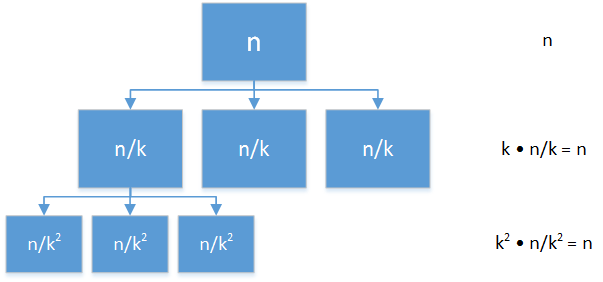
\includegraphics[scale=1.00]{figs/IO_II_3.png}
        \caption{Recursion tree for \emph{EM-MergeSort}}
        \label{fig:io-ii-3}
    \end{figure}
    The recursion can be denoted as $T(n) = \sum\limits_{i=1}^k T(n/k) + O(n)$
   Using $T(n)$ and the recursion tree it can be said that the running time of \emph{EM-MergeSort} is $l \cdot n$ where $l$ denotes the height of the tree. The height of the tree can be denoted as $l = \log_k n$. Therefore the running time of \emph{EM-MergeSort} is  $O(n\log n)$.

\item(3 points)
    In the proof of Theorem~6.2 we assumed that the algorithm only uses the blocks of the input array $A$, it does not use any additional storage in the external memory. Prove that without this assumption the same asymptotic lower bound holds.

    \emph{Hint:} Consider a permutation algorithm that \emph{does} use additional memory blocks. Show that the algorithm can be modified such that the assumption is satisfied---that is, such that all write operations are to blocks in $A$---while not increasing the number of \ios by more than a factor~3.
    
    \textbf{Answer:}
        
        I use the same symbol except for $X$ to denote the variables in my proof.
        
        Let's consider an algorithm {\sc Alg} that can solve this permutation problem in $Q~(Q<n^2)$ \ios in the worst case and does use additional storage in external memory. First, we need to define the output state differently from that used to prove Theorem~6.2. The external memory is formatted into blocks of size $B$. The input array occupies $n/B$ blocks in external memory. The extra storage that \alg can use consists of $C~(C<Q)$ blocks. This lead to at least $C$ empty blocks in external memory. The output state in \alg should now contain not only those blocks occupied by the array, but also the blocks in additional space. % Every such block should have a imaginary flag meaning they are used or not. (Used means it is used to store input or is written to by Write \ios). State in {\sc Alg} should be the state of all \emph{used} blocks.
        \begin{enumerate}
            \item[-] Similarly, we derive a bound on the total number of states that \alg must be able to reach to produce all possible permutations. There is one output state where $M=\phi$ and every element is in its right blocks (no matter in what order within the block), which occupy the same external memory space as input array again after all these permutations. The bound in \alg is different from that in Theorem~6.2 in that we need to choose $\frac{n}{B}$ blocks from $C+\frac{n}{B}$ blocks. Thus, the total number of different output state becomes:
            $$\binom{C+\frac{n}{B}}{\frac{n}{B}} \cdot \frac{n!}{(B!)^{n/B}}$$
            \item[-] The read operation defined in proof of Theorem~6.2 is still valid: after a read operation the number of the states increases by $\frac{n}{B}$ at most. (Suppose \alg doesn't read empty blocks because this is a movement-only model.)
            \item[-] The write operation would be different from that in the proof of Theorem~6.2. There are at most $n/B+C$ empty blocks available. Hence, a write operation in \alg increases the number of state by $\binom{M}{B}\cdot (\frac{n}{B}+C)$
        \end{enumerate}
        Follow similar procedure of proving Theorem 6.2:
        $$\binom{C+\frac{n}{B}}{\frac{n}{B}} \cdot \frac{n!}{(B!)^{n/B}} \leq (\frac{n}{B})^{Q/2} \cdot (\binom{M}{B}\cdot (\frac{n}{B}+C))^{Q/2}$$
        $$(Q/2) \cdot \log((n/B)\binom{M}{B}(n/B+C)) \geq \log(\binom{C+\frac{n}{B}}{\frac{n}{B}})+\log(\frac{n!}{(B!)^{n/B}})$$
        $$(Q/2) \cdot \log((n/B)\binom{M}{B}(n/B+C)) \geq \log(\frac{n!}{(B!)^{n/B}})$$
        Consider the left-hand side of the inequality above first, from the assumption that $n<B\sqrt{\binom{M}{B}}$, we can derive that:
        $$\frac{n}{B} < \binom{M}{B} \textrm{~and~} \frac{n}{B}+C<\binom{M}{B}$$
        $$3\log(\binom{M}{B}) > \log((n/B)\binom{M}{B}(n/B+C))$$
        Using the inequality $\binom{M}{B} \leq (\frac{eM}{B})^B$, we obtain
        $$\frac{3}{2}\log(\binom{M}{B})<3B\log(\frac{M}{B})$$
        From the proof of Theorem 6.2, we also use Stirling's approximation to bound the right-hand side as
        $$\log(\frac{n!}{(B!)^{n/B}}) = \Omega(n\log(n/B))$$
        Combining all above,
        $$Q \geq \frac{\Omega(n\log(n/B))}{3B\log(\frac{M}{B})}$$
        $$Q \geq \Omega((n/B)\log_{M/B}(n/B))$$
        Asymptotically, \alg has the same bound as the algorithm in Theorem 6.2.

\end{rlist}




%------------------------------------------------------------------------------
\renewcommand{\setnr}{IO.III}
\subsection*{Exercise Set I/O-Efficient III}
%------------------------------------------------------------------------------

\begin{rlist}

\item ($2 + 2$ points)
    Consider a balanced binary search tree $\tree$ with $n$ internal nodes that is stored in external memory. You may assume that $n=2^k-1$ for some integer~$k$, and that the tree is perfectly balanced.
    Hence, its depth is~$\log_2 (n+1)$.
    \begin{enumerate}
        \item[(i)]
            Describe blocking strategy that guarantees that any root-to-leaf path in $\tree$ can be traversed in $O(\log_B n)$. What is the relation of your blocking strategy to B-trees?
        \item[(ii)]
            Prove that for \emph{any} blocking strategy there will be a root-to-leaf path that visits $\Omega(\log_B n)$ blocks. To simplify the proof you may assume that the blocking strategy has the following property: for each block $b$, the nodes in $b$ form a connected part of $\tree$. This implies that whenever a root-to-leaf path leaves a block, it will not re-enter that block. 
    \end{enumerate}
    
    \textbf{Answer:}
    \begin{enumerate}
        \item[(i)]
    A blocking strategy for $O(\log_B n)$ \ios is storing a subtree up to a depth of $log_2 B$. Whereas any step in the root-to-leaf path is a new subtree. The root-to-leaf path is the depth of the tree which is $O(\log_2 n)$ divide it by the amount that can be reached per \io then the \io cost is $O(\frac{\log_2 n}{\log_2 B}) = O(log_B n)$
        
    
    This blocking strategy is comparable to a one of a B-tree where the branching degree k is set to 2.
    
    \item[(ii)]
    The blocking strategy in (i) is a optimal strategy for a perfectly balanced binary tree hence all paths will be of depth $log_2 B$. If the blocking strategy is changed to make a path longer and B stays the same, then another path must become shorter. Then for any blocking strategy there is always a root-to-leaf path that visits $\Omega(\log_B n)$ blocks.
    \end{enumerate} 
\item (2 points)
    The \io-efficient priority queue described above keeps a set $S^*$ in internal memory that contains $M/4$ elements when $S^*$ is created. The next $M/4$ operations are then performed on $S^*$, after which the elements that still remain in $S^*$ are inserted into the buffer tree (and $S^*$ is emptied). Someone suggests the following alternative approach: instead of only performing the next $M/4$ operations on $S^*$, we keep on performing \emph{Extract-Min} and \emph{Insert} operations on $S^*$ until $|S^*|=M$. Does this lead to correct results? Explain your answer.
    
    \textbf{Answer:}
    This won't lead to correct results. Inserting a key with priority higher than a priority that is still in external memory will create a temporary node position in $S^*$. After $M/4$ operation there's a flush that will place this node in the right position in $\tau_{buf}$. But if we continue to perform operations on $S^*$, the \emph{Extract-Min} operation can only guarantee that the node extracted has the minimal priority within $S^*$, not minimal among entire $\tau_{buf}$. 
        
    For example, the range of the priority in $S^*$ is $[1, 50]$, the range of the priority in the node remaining in $\tau_{buf}$ is $[51, 100]$. When inserting a key \textbf{K} with priority 60, it will first be inserted to $S^*$ in memory. Key \textbf{K} will not be extracted before $M/4$ operations because there's definitely other keys with lower priority. However, after $M/4$ operations, when all the keys loaded from the the external memory might be extracted, the algorithm will extract key \textbf{K}. This is wrong because \textbf{K}'s priority is~60 but there might be external keys with priority 55.

\item (4 points)
    A \emph{coloring} of an undirected graph~$\G=(V,E)$ is an assignment of colors to the nodes of $\G$ such that if $(v_i,v_j)\in E$ then $v_i$ and $v_j$ have different colors. Suppose that $\G$ is stored in the form of an adjacency list in external memory. Assume the maximum degree of any node in $\G$ is~$d_{\max}$. Give an algorithm that computes a valid coloring for $\G$ that uses at most $d_{\max}+1$ colors. Your algorithm should perform $O(\sort(|V|+|E|)$ \ios.
    
    \textbf{Answer:}
    First, we turn $\G$ into the {\sc dag} $\G^*$ by directing every edge $(v_i, v_j) \in E$ from the node with the smaller index to the node with the higher index. We do not have to do anything to the data, since the data is already by definition stored in a topological way in the external memory: we can just interpret the representation of $\G$ as a representation of $\G^*$.
    
    Define $C$ to be the set of $d_{\max}+1$ unique colours. Define $N_{in}(v_i)$ to be the set of all in-neighbours of $v_i$. Define the local function $f$ on the nodes as follow.
    \begin{itemize}
        \item
            If $|N_{in}(v_i)| = 0$ then $f(v_i)$ may be any color $c \in C$.
        \item
            If $|N_{in}(v_i)| > 0$ then $f(v_i)$ may be any color $c \in C \setminus f\left(N_{in}(v_i)\right)$.
    \end{itemize}
    
    It is easy to see that $\G$ is now colored in such a way that for every edge $(v_i, v_j) \in E$, the two nodes $v_i$ and $v_j$ have different colours, thus meeting the requirement. If a node $v_i$ has no in-neighbours, $f$ will give it per definition a colour unique to its in-neighbours. If a node $v_i$has one or more in-neighbours, $f$ will give it a colour unique to all its in-neighbours, since $C = d_{\max}+1 > d_{max} \geq |N_{in}(v_i)|$ proves that such a colour is always available from $C$. Because every node $v_i$ has a different colour than its in-neighbours, it must have a different colour than its out-neighbours have a different colour than their in-neighbour $v_i$.
    
c    Since every $f(v_i)$ can be computed in $O(\sort(1+|N_{in}(v_i)|))$ \ios, we can compute the colouring of $\G$ using $O(\sort(|V|+|E|))$ \ios, as proven in Theorem 7.2 of the lecture notes.
\end{rlist}

\end{document} 

